\documentclass[../main.tex]{subfiles}
\begin{document}
%%%%%%%%%%%%%%%%%%%%%%%%%%%%%%%%%%%%%%%%%%%%%%%%%%%%%%%%%%%%%%%%%%%%%%%%%%%%%%%%%%%%%
%%%%%%%%%%%%% Tree Traverse
%%%%%%%%%%%%%%%%%%%%%%%%%%%%%%%%%%%%%%%%%%%%%%%%%%%%%%%%%%%%%%%%%%%%%%%%%%%%%%%%%%%%%%%%% 
As the second Chapter related to trees, it is time for us to learn how to complete search a given tree and learn the different applications of trees as mentioned in Chapter~\ref{chapter_}. Same as a graph data structure, the first thing before thinking about any algorithms is to learn methods to traverse the tree. As in graph, there are two broad ways to iterate all nodes and edges in the tree, Depth-first-search(DFS) and Breath-first-search(BFS). Gladly, due to simpler structure the tree is and it has no cycles, the traverse of a tree is easier to implement than that of a general graph, because there are no cycles in the tree and it is not possible to reach a node from multiple directions. 

\paragraph{Tree Traversal} We first talk about general traversal of trees, first start with the free trees, which are just simplified version of graph search implementation without the state records. We mainly focus on the implementation of rooted trees and learn both recursive and iterative implementation. These contents will be shown in:
\begin{enumerate}
    \item Depth-first-search based Tree Traversal in Section~\ref{dfs_tree_traversal}.
    \item Breath-first-search based Tree Traversal in Section~\ref{bfs_tree_traversal}.
\end{enumerate} 

\paragraph{Applications} We then focus on the applications of trees, mainly with different types of search trees, include binary search tree (BST), segment tree, trie for string and order statistic trees. We would learn how to do search in these different trees and how to implement basic operations to make it a data structure such as insert, delete, and construction. 
\begin{enumerate}
    \item Binary Search Tree in Section~\ref{}.
    \item Segment Tree in Section~\ref{}.
    \item Trie for string in Section~\ref{}.
\end{enumerate}

\begin{figure}[h]
    \centering
    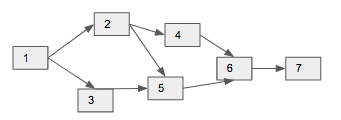
\includegraphics[width=0.6\columnwidth]{fig/example_graph.png}
    \caption{Example Graph vs converted tree, where we delete edge $3->5$ and $5->6$.}
    \label{example_graph_tree}
\end{figure}




\end{document}